\documentclass{article}
\usepackage[utf8]{inputenc}
\usepackage{hyperref}
\usepackage[letterpaper, portrait, margin=1in]{geometry}
\usepackage{enumitem}
\usepackage{amsmath}
\usepackage{booktabs}
\usepackage{graphicx}

\usepackage{hyperref}
\hypersetup{
colorlinks=true,
    linkcolor=black,
    filecolor=black,      
    urlcolor=blue,
    citecolor=black,
}
\usepackage{natbib}

\usepackage{titlesec}

\title{Homework 8}
\author{Roshani Bulkunde}
\date{April 2023}

\begin{document}

\maketitle
\begin{enumerate}
    \item Produce a yearly plot of the recycling rate for NYC and the controls to examine the effect of the recycling pause and the possibility of parallel trends.
    
    
    \begin{figure}[ht]
    \centering
    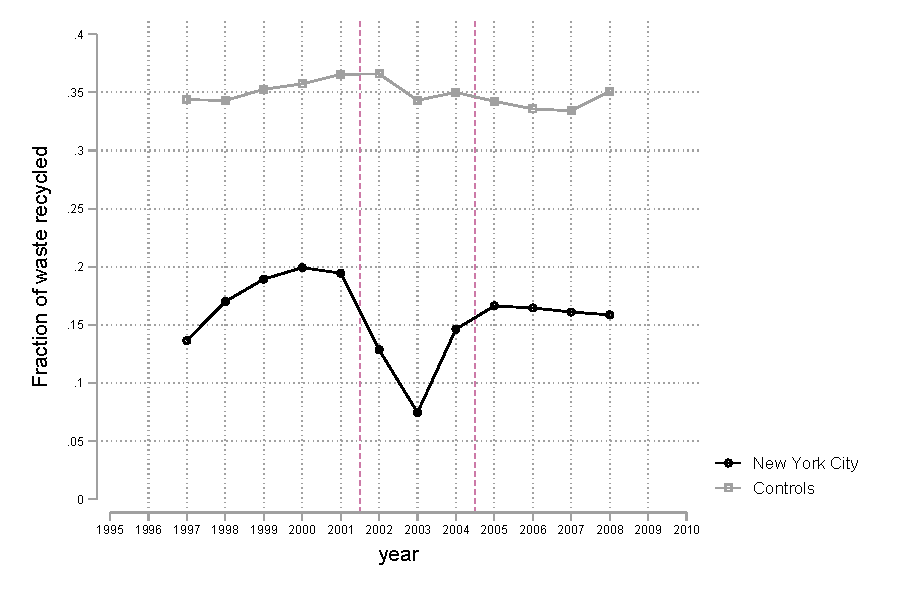
\includegraphics[scale = 0.7]{hw8_q1parallel.pdf}
    \caption{Plot of a scatterplot}
    \label{fig:hw8_q1parallel}
    \end{figure}

    \begin{figure}[ht]
    \centering
    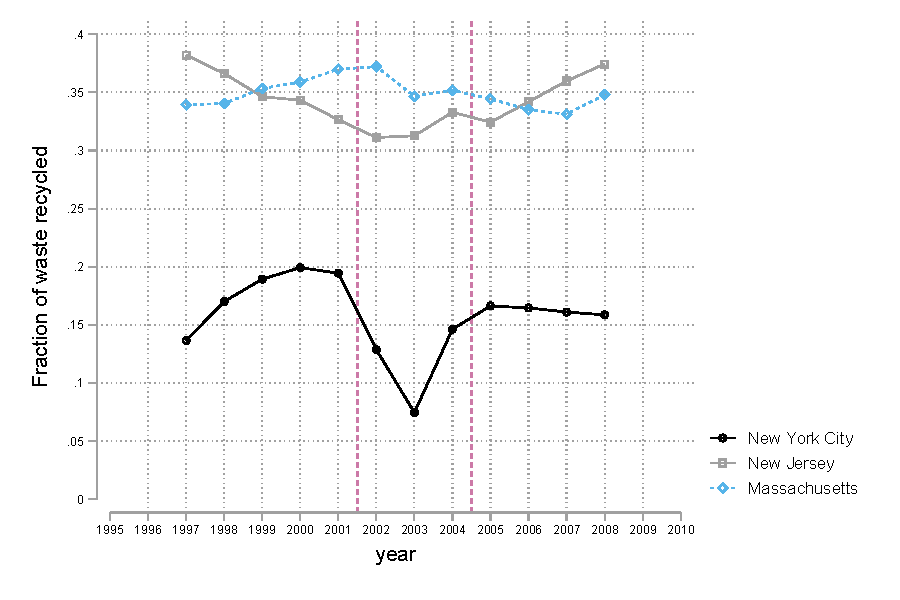
\includegraphics[scale = 0.7]{hw8_q1parallel_2.pdf}
    \caption{Plot of a scatterplot}
    \label{fig:hw8_q1parallel_2}
    \end{figure}

    


    \item Estimate the effect of the pause on the recycling rate in NYC using a TWFE regression and the data from 1997-2004. Cluster your standard errors at the region level. Report the average treatment effect estimate and the standard error.
          \item[Answer:] The average treatment effect estimate is -0.62 and the standard errors are 0.005
    


    \item Use the command sdid to estimate the synthetic DID version of the TWFE regression in equation 2. Report the estimated average treatment effect and the synthetic DID plot using the graph option.
       
    \begin{table}[ht]
    \centering
    {
\def\sym#1{\ifmmode^{#1}\else\(^{#1}\)\fi}
\begin{tabular}{l*{1}{c}}
\hline\hline
            &\multicolumn{1}{c}{(1)}\\
            &\multicolumn{1}{c}{recyclingrate}\\
\hline
interaction &      -0.064***\\
            &     (0.007)   \\
\hline
\(N\)       &        1680   \\
\hline\hline
\multicolumn{2}{l}{\footnotesize Standard errors in parentheses}\\
\multicolumn{2}{l}{\footnotesize * p<0.10, ** p<0.05, *** p<0.01}\\
\end{tabular}
}

    \caption{estimate the synthetic DID version of the TWFE regression}
    \label{tab:q3_sdid}
    \end{table}

    \begin{figure}[ht]
    \centering
    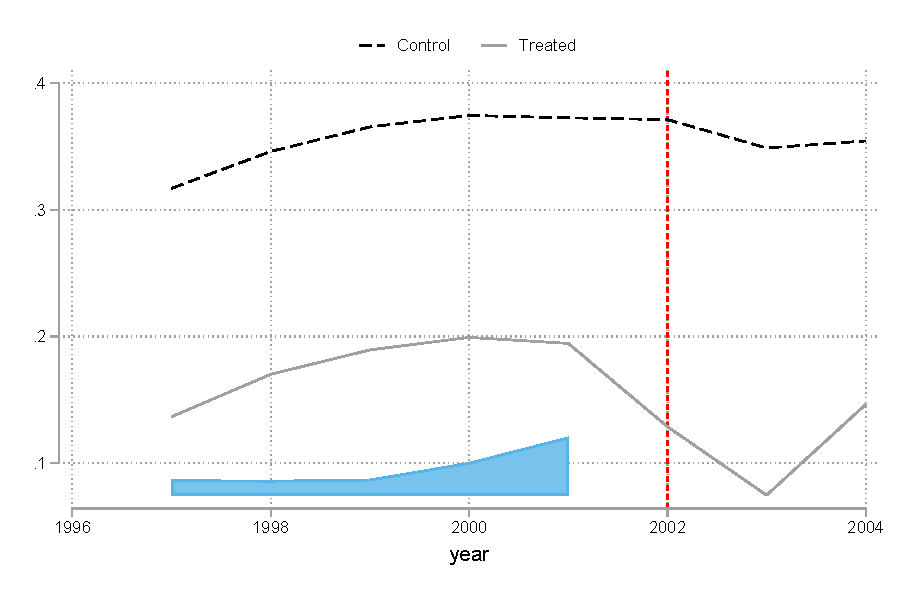
\includegraphics[scale = 0.7]{sdid_graphtrends2002.pdf}
    \caption{The synthetic DID plot}
    \label{fig:sdid_graphtrends2002}
    \end{figure}


    \item Using the full sample, estimate the following event study regression:
    \begin{align}
    Y_{i,t} &= \alpha_{i} + \gamma_{t} + \sum_{i} D_{i}.1(t = l) \beta_{l}+ \gamma X_{i,t}  + \epsilon_{i,t}
    \end{align}
    where  $D_{i}$ is a binary variable equal to one for New York City regions, 1(t = l) is an indicator function equal to one for year l, and $X_{i,t}$ are any time-varying controls you would like to include. Do not use a canned event study regression. Use reg, xtreg, or reghdfe. Report your results as a picture of the coefficient estimates of $\beta_{l}$ with confidence intervals derived from standard errors clustered at the region level (use coefplot). Note that you will need to generate treatment variables to estimate this regression.

    \begin{figure}[ht]
    \centering
    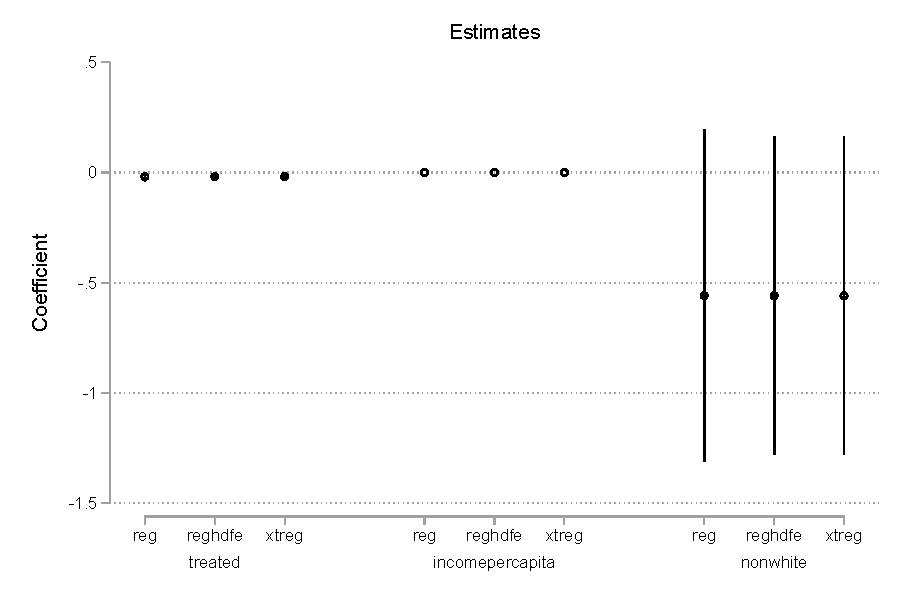
\includegraphics[scale = 0.7]{hw8_q4_coefplot.pdf}
    \caption{The coefficient estimates of $\beta_{l}$ with confidence intervals derived from standard errors clustered at the region level}
    \label{fig:hw8_q4_coefplot}
    \end{figure}

    \newpage

    


    \item Use the commands synth and synth\_runner to generate synthetic control estimates of the dynamic treatment effects. Generate the synthetic control estimates using whichever matching variables you see as most appropriate. Use placebo inference. Report:
    
    
    \begin{enumerate}
        \item The plot of raw outcomes for treated and control groups over time.
         \begin{figure}[ht]
        \centering
        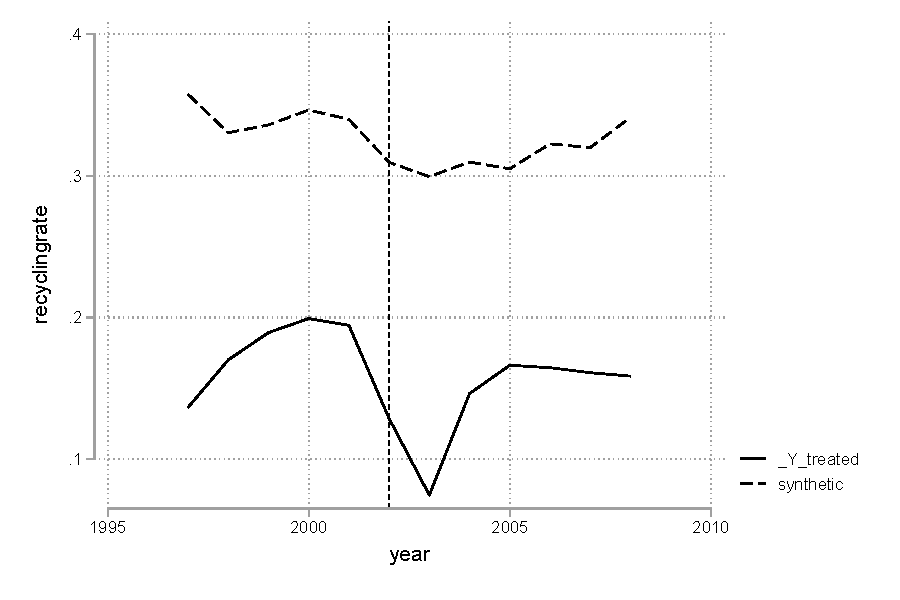
\includegraphics[scale = 0.7]{hw8_q5a_synth.pdf}
        \caption{Raw outcomes for treated and control groups over time}
        \label{fig:hw8_q5a_synth}
        \end{figure}
        

        \item The plot of raw outcomes for the treated group and synthetic control group over time.

        
            \begin{figure}[ht]
            \centering
            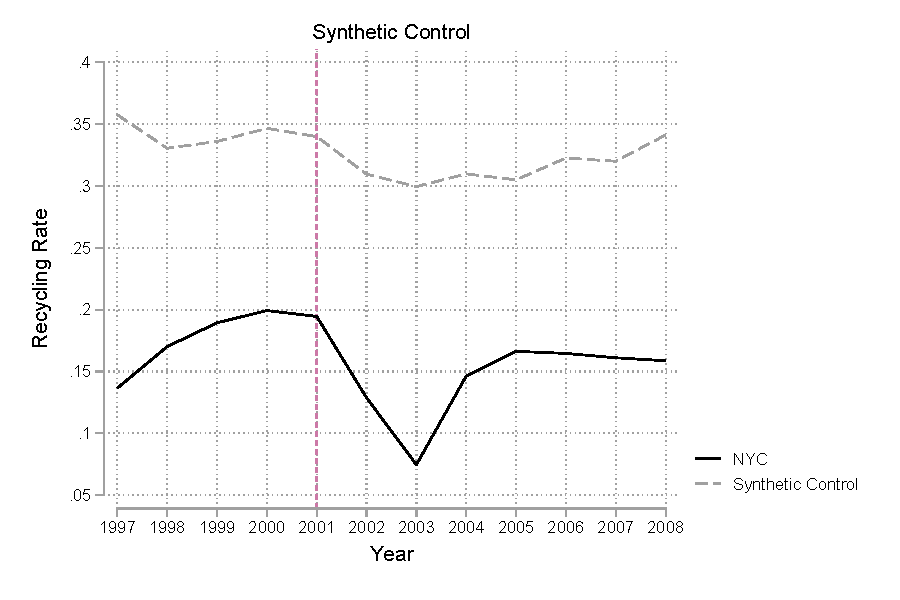
\includegraphics[scale = 0.7]{hw8_q5btc.pdf}
            \caption{Raw outcomes for the treated group and synthetic control group over time}
            \label{fig:hw8_q5btc}
            \end{figure}

        
            \begin{figure}[ht]
            \centering
            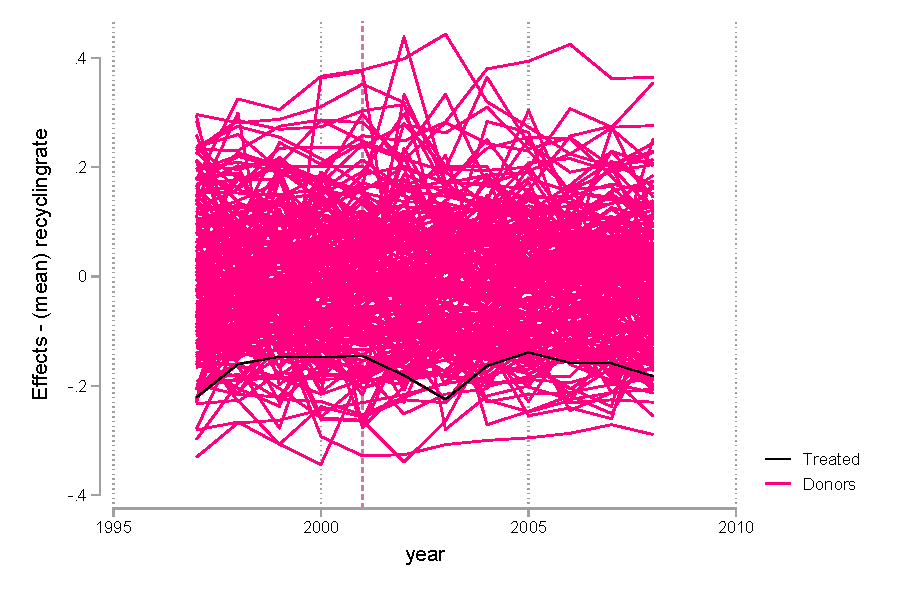
\includegraphics[scale = 0.7]{5b_effects.pdf}
            \caption{Effect}
            \label{fig:5b_effects}
            \end{figure}

        
            \begin{figure}[ht]
            \centering
            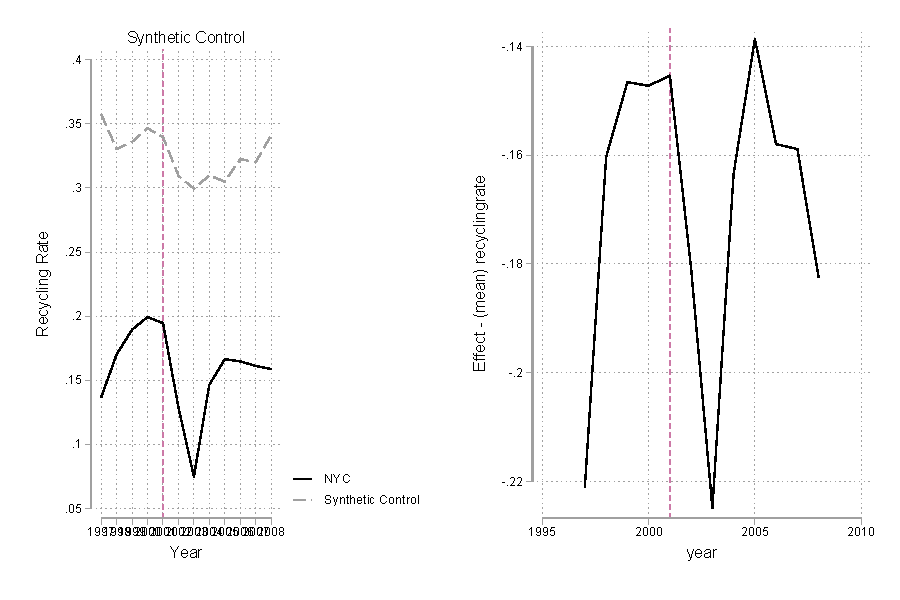
\includegraphics[scale = 0.7]{5b_combine_effecttc.pdf}
            \caption{Raw outcomes for treated and control groups over time}
            \label{fig:5b_combine_effecttc}
            \end{figure}
            
           
            \begin{figure}[ht]
            \centering
            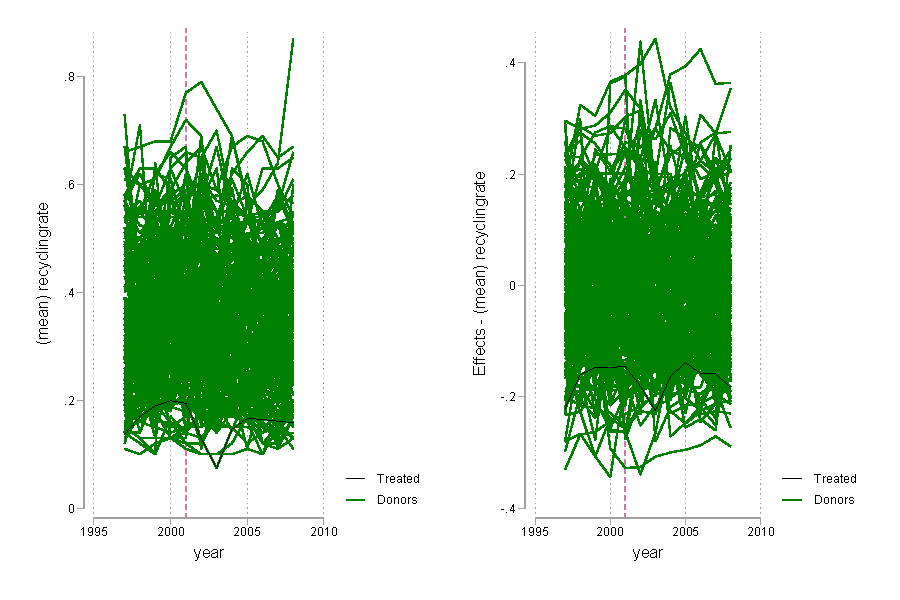
\includegraphics[scale = 0.7]{hw8_q5raw.pdf}
            \caption{Raw outcomes for treated and control groups over time}
            \label{fig:hw8_q5raw}
            \end{figure}

        
       

        





       
        
        \item The plot of estimated synthetic control effects and placebo effects over time.
        \begin{figure}[ht]
        \centering
        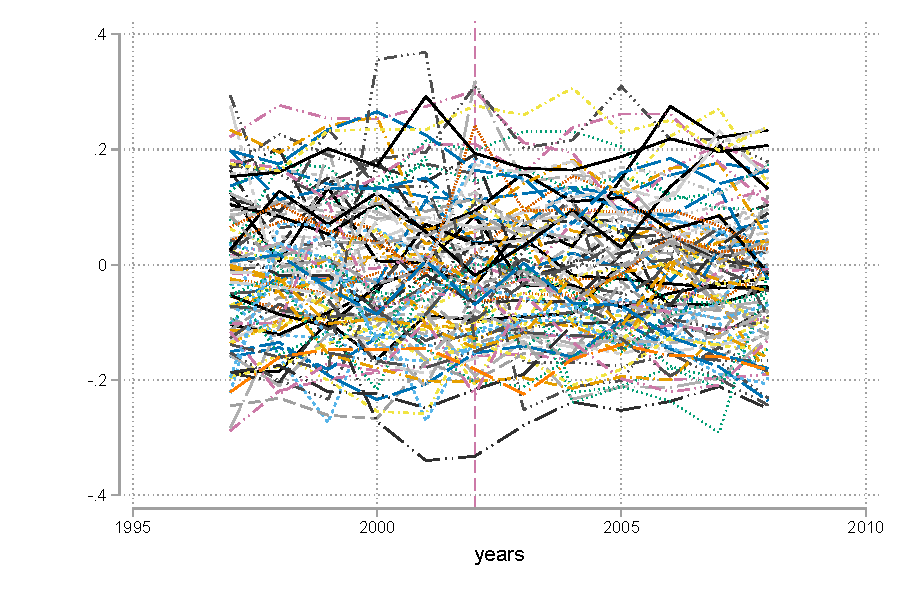
\includegraphics[scale = 0.7]{hw8_q5c.pdf}
        \caption{The plot of estimated synthetic control effects and placebo effects over time}
        \label{fig:hw8_q5c}
        \end{figure}

        

        


        
        
    \end{enumerate}
    
\end{enumerate}


\end{document}

